\documentclass[11pt]{article}
%\usepackage[round]{natbib}
\usepackage{setspace} 
\usepackage{dsfont}
\usepackage{amsfonts}
\usepackage{amsmath}
\usepackage{subcaption}
\usepackage{paralist}
%\usepackage{subfig}
\usepackage{times}
\usepackage{latexsym}
\usepackage{graphicx}
\usepackage[T1]{fontenc}
\usepackage{tikz}
\usepackage{url}
\usepackage{pgfplotstable}
\usepackage{titlesec}
\usepackage{color}
\usepackage{lipsum,adjustbox}
\usepackage[font={small}]{caption}
\usetikzlibrary{positioning}

\makeatletter
\newcommand{\@BIBLABEL}{\@emptybiblabel}
\newcommand{\@emptybiblabel}[1]{}
%\makeatother
\usepackage[hidelinks]{hyperref}


\usepackage{acl2012}
\graphicspath{{./plots/}}
\newcommand{\com}[1]{}
\newcommand{\oa}[1]{\footnote{\color{red}OA: #1}}
\newcommand{\lc}[1]{\footnote{\color{green}LC: #1}}

\begin{document}

%\author{
%  Leshem Choshen\textsuperscript{1} and Omri Abend\textsuperscript{2} \\
%  \textsuperscript{1}School of Computer Science and Engineering,
%  \textsuperscript{2} Department of Cognitive Sciences \\
%  The Hebrew University of Jerusalem \\
%  \texttt{leshem.choshen@mail.huji.ac.il, oabend@cs.huji.ac.il}\\
%}

\section*{Improved Methodology for Reference-based Evaluation in 
	Grammatical Error Correction}

% Error correction 
% evaluation in error correction and its centrality
% faithfulness to the source meaning is important, and this has been noted but prev work, and evaluation is geared towards it
% gap in evaluation: however, steps taken to ensure conservativeness in fact push towards formal conservativism by their definition (theoretical claim about the measure)
% this may result in systems that make few changes. indeed we find that this is the case (empirical claim about systems)

% we pursue two approaches to overcome this bias.

% 1. increasing the number of references. this has been proposed before and pursued with m=2, but no assessment of its sufficiency or its added value over m=1 has been made. In order to address this gap we first charachterize the distribution of possible corrections for a sentence. We leverage this characterization to characterize the distribution of the scores as a function of $m$, and consequently assess the biases introduced by taking $m=1,2$ as with previous approaches. 
% We find that taking these values of $m$ drammatically under-estimate the system scores. 
% We back our analysis of these biases with an analysis of the variance of these estimators.
% We analyze the two commonly used scores, the M2 score often used for evalauted, and the accuracy score commonly used in training.

% 2. we note that in fact the important factor is semantic conservativism and explore means to directly assess how semantically conservative systems here through the use of semantic annotation. 
% We use the UCCA scheme as a test case, motivated by HUME.
% First question: is it well-defined on learner language. it is.
% Second question: are corrections in fact semantically conservate? to show that, we need to verify that the corrections make few (if any) semantic changes. our results indicate that this is the case: we show that the corrections are similar in (UCCA) structure to the source.

% conclusion (not in intro): we tried to use semantic similarity to improve systems. this is difficult due to semantic conservatism. we expect this will be in issue once evaluation is improved. future work.
% also future work: use multiple references in training (did people do that?)

% sections:
% 1. Introduction
% 2. Formal conservativism in GEC
% 3. First approach: Multiple References
% 3.1. A Distribution of Corrections
% 3.2. Scores (M2, accuracy index, accuracy exact)
% 3.3. Data
% 3.4. Bias of the Scores (setup + results)
% 3.5. Variance of the Scores (setup + results)
% 4. Second approach: Semantic Similarity
% 4.1. Semantic Annotation of Learner Language (prev work)
% 4.2. UCCA Scheme (see HUME)
% 4.3. Similarity Measures (including prev work of elior)
% 4.4. Empirical Validation: IAA, semantic conservativism vs. gold std
% 5. Conclusion

Grammatical Error Correction (GEC) is a challenging research field, which interfaces with many other application areas of linguistics. The field is receiving considerable
interest recently, notably through the GEC-HOO \cite{dale2011helping,dale2012hoo},
CoNLL shared tasks \cite{kao2013conll,ng2014conll}.
Within GEC, considerable effort has been placed on system evaluation,
which is notoriously difficult,
much due to the many valid corrections each source sentence may have \cite{tetreault2008native,madnani2011they,chodorow2012problems,dahlmeier2012better}.

An important criterion in the evaluation of GEC systems (henceforth, {\it correctors})
is their ability to generate corrections that are faithful to meaning of the source. In fact, many would prefer
a somewhat cumbersome or even an occasionally ungrammatical correction over a correction
that alters the meaning of the source \cite{brockett2006correcting}.
As a result, often when compiling gold standard corrections for the task,
annotators are instructed to be conservative in their corrections, e.g. in NUCLE \cite{dahlmeier2013building} and the Treebank of LL\cite{yannakoudakis2011new}.
A recent attempt to formally capture this precision/recall asymmetry has
been the shift from using $F_1$ to $F_{0.5}$, where Precision is
emphasized over Recall, as a common evaluation measure
in GEC \cite{dahlmeier2012better}.

However, favoring precision over recall may lead to reluctance of correctors to make any changes.
Using a single reference correction (a common practice in GEC) compounds this problem,
as systems are not only penalized more for making an incorrect change, but are often penalized for any correct change not found in the reference.

We present results that indicate that current state of the art systems suffers
from over-conservatism. Evaluating the output of 15 state
of the art GEC systems that participated
in the recent CoNLL2014 shared task, we find that all of them
substantially under-predict corrections relative to the gold standard. 

We pursue two approaches to address this gap, proposing
improved reference-based protocols to decrease penalties of valid correction. Thus, avoiding over-conservatism.
First, we study the effect of increasing the amount of references
(henceforth, $M$).
While previous evaluation explored the case of $M=2$,
no empirical assessment has been carried out, of its sufficiency
or its added value over $M=1$.
In our experiments we estimate the number of corrections necessary
to cover the bulk of the distribution of possible corrections.
We then consider two measures for
assessing the validity of a proposed correction relative to a set of references,
and characterize the distribution of their scores as a function of $M$.
We find that assessment based on $M=1$ or $M=2$ dramatically under-estimate
the true performance. 
We conclude with an analysis of
the statistical significance of these evaluation protocols.

Second, we pursue an alternative way by developing a semantic measure based
on the similarity of their {\it semantic} structures.
We define a measure, using the typology inspired UCCA scheme \cite{abend2013universal} as a
test case.
In order to assess the feasibility of this approach, we annotate a
section of the NUCLE
parallel corpus. Our results support the feasibility of the proposed approach,
by showing that semantic structural annotation can be consistently applied
to LL and that manually compiled references do indeed
have similar semantic structures to those of their source sentences.

The two approaches address the insufficiency of using too few references from
complementary angles. 
The first attempts to cover the bulk of the distribution of possible
corrections for a sentence, while the second
uses semantic instead of string similarity, in order to abstract away
from some of the formal variation between different valid corrections.
 
\bibliographystyle{acl2012}
\bibliography{propose}

\appendix

 \begin{figure}
 	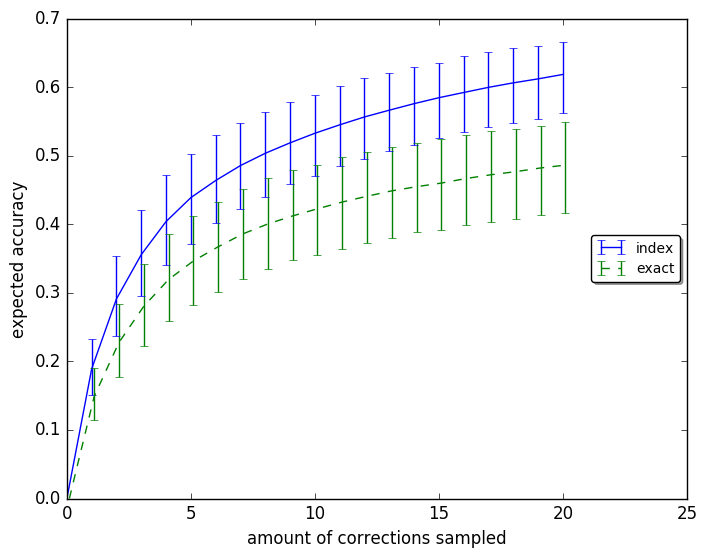
\includegraphics[width=8cm]{repeat_1000_accuracy}
 	\caption{Mean accuracy values for perfect correctors with different number of references. Lines shows accuracy based on exact match and exact index match, match iff the same words were deleted added or changed.} \label{fig:accuracy_vals}
 \end{figure}



\vspace*{-\baselineskip}
\begin{table}[h!]
	\centering
	\singlespacing
	\begin{tabular}{c|c|c|c|c}
		Annotator & Edit & Fully aligned & Top down & Token analysis
		\\
		\hline
		Same& 323.16 & 0.78 & 0.79 & 0.85
		\\
		Different & 209.55 & 0.85 & 0.87 & 0.89
		\\
		\end{tabular}
		\caption{Different UCCA distance measures between LL and corrected parallel paragraphs. The scores are quite similar to the IAA, which means distances are indeed low.\label{tab:Distances}}
	\end{table}
\end{document}
